\documentclass[10pt]{article}

\usepackage[margin=0.62in]{geometry}
\usepackage{booktabs}
\usepackage{tabularx}
\usepackage{microtype}
\usepackage{xcolor}
\usepackage[hidelinks]{hyperref}
\usepackage{tikz}
\usetikzlibrary{arrows.meta}

\setlength{\parindent}{0pt}
\setlength{\parskip}{4pt}
\setlength{\tabcolsep}{3.5pt}
\renewcommand{\arraystretch}{1.08}

\title{Deep Learning: Final Project\\
Image Geolocation Challenge}
\author{Arham Shahzad}
\date{}

\begin{document}
\maketitle
\vspace{-1.5em}

\section*{Experimental setup}

I used the same country-stratified 80/20 train--validation split
($9{,}408/2{,}352$ images, random state 42) throughout the experiments. The
backbone was ImageNet-pretrained MobileViTV2-1.0 \cite{mobilevitv2}; the final
108-output model has 4,444,245 parameters. Model selection used validation
median Haversine distance, with patience-four early stopping. Table
\ref{tab:experiments} records the development path rather than only the
successful final configuration.

\begin{table}[h]
\centering
\caption{Experiment progression. ``Raw $\rightarrow$ tuned'' separates the
trained checkpoint from validation-selected inference calibration.}
\label{tab:experiments}
\small
\begin{tabularx}{\textwidth}{@{}c p{0.27\textwidth} p{0.13\textwidth} X@{}}
\toprule
\# & Experiment & Median (km) & Main observation \\
\midrule
1 & Normalised latitude/longitude regression & 625.8 & Direct MSE regression learned a broad geographic compromise but remained inaccurate. \\
2 & Cartesian $(x,y,z)$ regression & Not retained & Removing longitude discontinuity did not provide a useful improvement over direct regression. \\
3 & Country auxiliary head & 516.9 & Country supervision gave the shared backbone a stronger coarse geographic signal. \\
4 & Post-hoc country-centre blend & 397.5 & Probability-weighted country centres were more reliable than the coordinate head. \\
5 & Integrated country blend & 373.1 & Training through the blended coordinate aligned the loss with the inference calculation. \\
6 & 64 global geographic cells & 357.7 & Finer regions improved locality, although direct-coordinate refinement still added noise. \\
7 & Cell-only fine-tuning and temperature & $320.9\rightarrow304.1$ & Removing direct coordinates helped; sharper cell probabilities improved the median but increased some large errors. \\
8 & Country-gated country-specific cells & $283.0\rightarrow270.5$ & Soft country probabilities suppressed geographically inconsistent cells without hard exclusion. \\
9 & Equal-population cell construction & 278.3 & More even class counts did not outperform ordinary country-specific cells; some cells lost geographic compactness. \\
10 & Capacity-constrained K-means cells & 280.8 & A better balance between equal counts and compactness gave an oracle median of 80.2 km, but prediction remained the bottleneck. \\
11 & 384-pixel training & $233.5\rightarrow224.6$ & Higher resolution produced the largest architectural gain by preserving small visual cues. \\
12 & 512-pixel fine-tuning and multi-resolution inference & $208.5\rightarrow\mathbf{199.1}$ & Averaging 384/512 logits improved all four validation metrics without adding parameters. \\
\bottomrule
\end{tabularx}
\end{table}

\section*{What failed and what changed}

\textbf{Regression was the wrong abstraction.}
The first models asked a small network to infer two continuous numbers directly.
Normalisation made optimisation stable, and Cartesian targets removed the
longitude wrap-around, but neither supplied useful geographic structure. The
country experiment exposed the main failure mode: correct-country predictions
had much smaller errors than incorrect-country predictions. This motivated
using classification probabilities as part of the coordinate calculation,
rather than treating classification only as an auxiliary loss.

\textbf{Increasing geographic structure improved localisation.}
Country centres were robust but too coarse, so I replaced them with geographic
cells, following the general classification-based view of image geolocation
used by PlaNet \cite{planet}. For cell $j$, the final model computes
\[
\tilde p_j =
\frac{p(\mathrm{cell}_j)\,p(\mathrm{country}(j))}
{\sum_k p(\mathrm{cell}_k)\,p(\mathrm{country}(k))},
\qquad
\hat{\mathbf y}=\sum_j \tilde p_j\mathbf c_j,
\]

\begin{figure}[h]
\centering

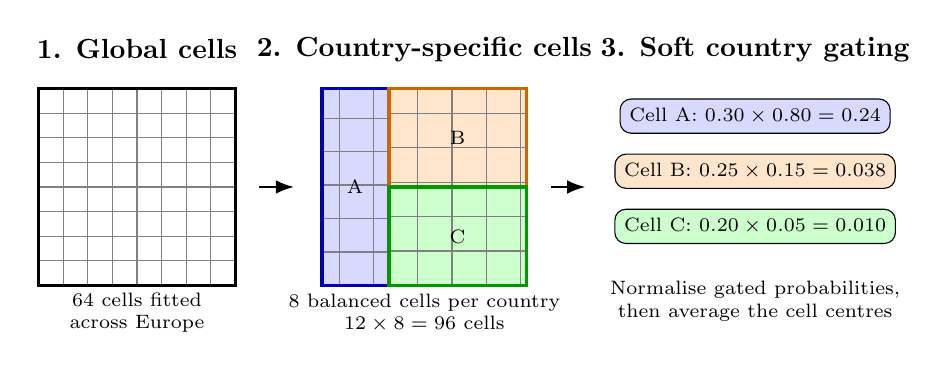
\begin{tikzpicture}[
    font=\scriptsize,
    >=Latex,
    panel/.style={
        draw,
        thick,
        minimum width=2.5cm,
        minimum height=2.5cm
    },
    arrow/.style={
        ->,
        thick,
        shorten >=3pt,
        shorten <=3pt
    }
]

% Panel 1: 64 global cells
\node[
    font=\bfseries
] at (1.25, 3.0) {
    1. Global cells
};

\draw[
    step=0.3125,
    gray,
    thin
] (0,0) grid (2.5,2.5);

\draw[
    thick
] (0,0) rectangle (2.5,2.5);

\node[
    align=center
] at (1.25,-0.35) {
    64 cells fitted\\
    across Europe
};


% Arrow 1
\draw[
    arrow
] (2.7,1.25) -- (3.35,1.25);


% Panel 2: country-specific cells
\node[
    font=\bfseries
] at (4.9,3.0) {
    2. Country-specific cells
};

% Country A
\fill[
    blue!15
] (3.6,0) rectangle (4.45,2.5);

\draw[
    step=0.425,
    gray,
    thin
] (3.6,0) grid (4.45,2.5);

\draw[
    blue!70!black,
    very thick
] (3.6,0) rectangle (4.45,2.5);

% Country B
\fill[
    orange!20
] (4.45,1.25) rectangle (6.2,2.5);

\draw[
    step=0.4375,
    gray,
    thin
] (4.45,1.25) grid (6.2,2.5);

\draw[
    orange!80!black,
    very thick
] (4.45,1.25) rectangle (6.2,2.5);

% Country C
\fill[
    green!20
] (4.45,0) rectangle (6.2,1.25);

\draw[
    step=0.4375,
    gray,
    thin
] (4.45,0) grid (6.2,1.25);

\draw[
    green!60!black,
    very thick
] (4.45,0) rectangle (6.2,1.25);

\node at (4.02,1.25) {A};
\node at (5.32,1.88) {B};
\node at (5.32,0.62) {C};

\node[
    align=center
] at (4.9,-0.35) {
    8 balanced cells per country\\
    $12 \times 8 = 96$ cells
};


% Arrow 2
\draw[
    arrow
] (6.4,1.25) -- (7.05,1.25);


% Panel 3: country gating
\node[
    font=\bfseries
] at (9.1,3.0) {
    3. Soft country gating
};

\node[
    draw,
    rounded corners,
    fill=blue!15,
    minimum width=3.4cm
] at (9.1,2.15) {
    Cell A: $0.30 \times 0.80 = 0.24$
};

\node[
    draw,
    rounded corners,
    fill=orange!20,
    minimum width=3.4cm
] at (9.1,1.45) {
    Cell B: $0.25 \times 0.15 = 0.038$
};

\node[
    draw,
    rounded corners,
    fill=green!20,
    minimum width=3.4cm
] at (9.1,0.75) {
    Cell C: $0.20 \times 0.05 = 0.010$
};

\node[
    align=center
] at (9.1,-0.20) {
    Normalise gated probabilities,\\
    then average the cell centres
};

\end{tikzpicture}

\caption{
Schematic progression from global geographic cells to
country-specific cells and soft country gating. The country
prediction does not alter the cell boundaries; it increases
or suppresses each cell's probability before the final
coordinate is calculated.
}

\label{fig:cell_progression}
\end{figure}

where $\mathbf c_j$ is the cell centre. This soft gate was preferable to hard
country selection because a wrong country prediction does not eliminate every
alternative. The loss combined coordinate MSE with country and cell
cross-entropy, each weighted by 0.01, so coordinate error propagated through
both probability heads.

Balancing cell populations was not automatically beneficial. The first balanced
partition improved class counts but produced less coherent regions and a worse
score. Capacity-constrained K-means, applied separately within each country and
with longitude scaled by mean latitude, produced equal-sized yet more compact
cells. Its 80.2 km oracle median showed that cell resolution was no longer the
main limitation: confusing cells was.

\textbf{Image resolution mattered more than further cell tuning.}
After several cell variants produced only small changes, increasing resolution
from the pretrained 256-pixel setting to 384 pixels reduced the raw median from
280.8 to 233.5 km. Fine-tuning the best checkpoint at 512 pixels reduced it to
208.5 km. This suggests that road signs, markings, poles, vegetation and
architectural details had been lost during lower-resolution preprocessing.

The final inference pass evaluates the same weights at 384 and 512 pixels,
averages their logits equally, and applies temperatures 0.25 (country) and 0.75
(cell). This gave a validation mean of 497.7 km, median of 199.1 km, 50.04\%
within 200 km and 78.61\% within 750 km. The improvement from multi-resolution
inference was small (201.0 to 199.1 km) but consistent across every reported
metric and required no additional parameters.

\section*{Limitations and conclusion}

Temperatures and resolution weights were chosen on the same validation split,
so the final 199.1 km estimate may contain mild post-processing overfit. I
therefore stopped after a small, coarse search rather than tuning fractional
values. The mean remains much larger than the median, indicating occasional
wrong-country or distant-cell failures. Nevertheless, the experiments show a
clear result: under a strict parameter budget, structured region probabilities
and higher-resolution inputs were substantially more effective than direct
coordinate regression. The final system reduced the validation median from
625.8 to 199.1 km while keeping a single 4.44M-parameter backbone.

\begin{thebibliography}{9}
\small
\bibitem{mobilevitv2}
S. Mehta and M. Rastegari,
``Separable Self-attention for Mobile Vision Transformers,''
\emph{arXiv:2206.02680}, 2022.

\bibitem{planet}
T. Weyand, I. Kostrikov, and J. Philbin,
``PlaNet---Photo Geolocation with Convolutional Neural Networks,''
in \emph{European Conference on Computer Vision (ECCV)}, 2016.
\end{thebibliography}

\end{document}
